%%%% OPTION
%% Change class according to your needs
%%  - article (no chapter)
%%  - report
%%  - etc.
\documentclass{article}


\IfFileExists{ifxetex.sty}{%
  \usepackage{ifxetex}%
}{%
  \newif\ifxetex
  \xetexfalse
}
  \ifxetex

\usepackage{fontspec}
\usepackage{xltxtra}
\setmainfont{DejaVu Serif}
\setsansfont{DejaVu Sans}
\setmonofont{DejaVu Sans Mono}
\else
\usepackage[T1]{fontenc}
\usepackage[utf8]{inputenc}
\fi
\usepackage{fancybox}
\usepackage{makeidx}
\usepackage{cmap}
\usepackage{url}
\usepackage{eurosym}

\usepackage[hyperlink]{sysfera}



%%%%
%% TODO:
%%  - ajouter une macro pour mettre l'objet du document
%%  - faire les footers avec l'adresse et tels de SysFera
%%  - enlever un max de paquets docbook


%%%%%%%%%%%%%%%%%%%%%%%%%%%%%%%%%%%%%%%%%%%%%%%%%%%%%%%%%%%%%%%%%%%%%%
%                            CONFIGURATION                           %
%%%%%%%%%%%%%%%%%%%%%%%%%%%%%%%%%%%%%%%%%%%%%%%%%%%%%%%%%%%%%%%%%%%%%%
% Use the following macros to configure your document
%%%%%%%%%%%%%%%%%%%%%%%%%%%%%%%%%%%%%%%%%%%%%%%%%%%%%%%%%%%%%%%%%%%%%%
%%%% OPTION
%% Change language: fr/en
%%  - for French: use french in babel, and fr in \setupsysferalocale
%%  - for English: use english in babel, and en in \setupsysferalocale

\usepackage[french]{babel}
\setupsysferalocale{fr}
\frenchbsetup{CompactItemize=false} % Fix itemize clash 
\usepackage{enumitem}
%%%% OPTION
%% Title and author of the document
\title{Utilisation des APIM}
\author{K. Coulomb}

%%%% OPTION
%% Document reference
%% Use command \SFdocumentreference to set the document reference.
%% Latter on, you can use the \SFthisdocument macro to retrieve
%% this reference.
\SFdocumentreference{PROCESS}
\SFprojectname{VISHNU}
\SFprojectleader{E.P. Capo-Chichi}
\SFclient{EDF}


%%%% OPTION
%% Release information. If the argument is not empty, then a box with
%% the content of the argument will be visible at the top of the document
%\SFreleaseinfo{Réalisé} % will show "Travail en cours" at the
                                 % top of the page
%\SFreleaseinfo{} % won't show anything

%%%% OPTION
%% Draft watermark. You can also show a grey watermak on all pages of
%% your document using the following command.
%\showwatermark{DRAFT}


%%%% OPTION
%% Add a logo into the header.
%% First parameter sets the width of the image relatively to the
%% \textwidth
%% Second parameter is the path to the image
% \SFsetheadlogo{.25}{fig/logosysfera.pdf}

%%%% OPTION
%% Collaborators:
%% You can redefine the Indexation of the document using the following command:
\renewcommand{\SFindexation}{
  \begin{SFindtable}
    \SFinditem{\writtenby}{K. Coulomb}{04 avril 2012}
%    \SFinditem{\verifiedby}{E.P. CapoChichi}{23 f\'evrier 2012}
%    \SFinditem{\approvedby}{E.P. CapoChichi}{23 f\'evrier 2012}
  \end{SFindtable}
}
% \renewcommand{\SFindexation}{} % disable this table


%%%% OPTION
%% Revision History Table:
%% Add a new \SFrevitem entry for adding a new entry in the revision
%% history table.
\renewcommand{\SFrevhistory}{
\begin{SFrevtable}
  \SFrevitem{1}{02/04/2012}{Premiere version}{K. Coulomb}
\end{SFrevtable}
}
% \renewcommand{\SFrevhistory}{} % disable this table


%%%% OPTION
%% References Table
%% Add a new \SFrefitem entry for adding a new entry in the list of
%% reference documents.
%\renewcommand{\SFreferenceTable}{
%\begin{SFreftable}
%  \SFrefitem{ref1}{techDocument}{Ce document}
%  \SFrefitem{ref2}{techDocument}{Ce document}
%\end{SFreftable}
%}
\renewcommand{\SFreferenceTable}{} % disable this table

%%%% OPTION
%% Authorization Table
%% Add a new \SFauthviewitem entry for adding a new entry in the list of
%% authorized users.
\renewcommand{\SFauthview}{
\begin{SFauthviewtable}
  \SFauthviewitem{SysFera}{L'équipe VISHNU}
\end{SFauthviewtable}
}
% \renewcommand{\SFauthview}{} % disable this table
%%%%%%%%%%%%%%%%%%%%%%%%%%%%%%%%%%%%%%%%%%%%%%%%%%%%%%%%%%%%%%%%%%%%%%
%                           /CONFIGURATION                           %
%%%%%%%%%%%%%%%%%%%%%%%%%%%%%%%%%%%%%%%%%%%%%%%%%%%%%%%%%%%%%%%%%%%%%%


\makeindex
\makeglossary


\begin{document}

\frontmatter % do not disable, this is used for page numbering
\maketitle % do not disable, otherwise you won't have any title
%%%% OPTION
\tableofcontents % comment to disable the table of contents
\mainmatter % do not disable, this is used for page numbering

%%%%%%%%%%%%%%%%%%%%%%%%%%%%%%%%%%%%%%%%%%%%%%%%%%
%% SECTION INTRO
%%%%%%%%%%%%%%%%%%%%%%%%%%%%%%%%%%%%%%%%%%%%%%%%%%

\section*{Introduction}
Ce document a pour but de présenter un apperçu global des process utilisés dans VISHNU pour générer tout les documents.
Il ne rentre pas dans les détails de qui sert à quoi, il présente juste la séquence des actions à faire pour être à jour dans VISHNU.

\section*{Le process global} 
Le process suivant ne tient pas compte des multiplicités (par exemple pour les specs chaque module a son fichier astah de spec). Il indique l'ensemble des actions.
Les numéros associés servent de référence dans le diagramme de séquence. Sur ce diagramme, les tâches sont découpées de manière aussi unitaire que possible.
\begin{itemize}
\item Mise à jour des fichiers astah STB (1)
\item Implémenter la couche WS (2)
\item Mise à jour du fichiers astah archi (3)
\item Mise à jour du fichiers astah design (4)
\item Mise à jour du fichiers astah data (5)
\item Création du fichier ecore (6)
\item Création du fichier apim, en le liant au ecore (7)
\item Utilisation de emf4cpp pour générer les classes de données C++ (8)
\item Utilisation du générateur de documentation API (9)
\item Utilisation du générateur de documentation manpage (10)
\item Utilisation du générateur de WSDL (11)
\item Utilisation du générateur de STB (12)
\item Utilisation du générateur de SpecGen (13)
\item Mise à jour du userman (14)
\item Mise à jour de l'adminman (15)
\item Génération du userman (16)
\item Génération de l'adminman (17)
\item Génération de la doc WS à partir des WSDL (18)
\item Mise à jour du plan du test (19)
\item Codage C++ des clients/serveurs (20)
\item Mise à jour des mappers (21)
\item Eventuellement, mettre à jour les exporteurs (pas si uniquement shell) (22)
\item Modifier le fichier swig (vishnu.i) (23)
\item Compiler avec swig/java/python pour générer les fichiers de generated (24)
\item Utilisation du générateur de documentation CLI (25)
\item Mise à jour du fichiers astah *MS (26)
\item Mise à jour du fichiers SpecGen-template (27)
\item Mise à jour du fichiers STB-template (28)
\item Mise à jour du fichiers api-template (29)
\item Mise à jour du fichiers cli-template (30)
\item Codage C++ des tests (31)
\item Générer le fichier design d'un module (32)
\item Création du fichier apim internal (33)
\item Passer les tests (34)
\item Ecrire le rapport de test (35)
\item Intégrer les tests en test automatiques hudson (36)
\item Regénérer les jars (37)
\item Mettre les fichiers swig java dans les jars du dépot eclipse (38)
\item Récupérer les dépots GIT (39)
\item Configurer son eclipse pour supporter les ecore/apim (40)
\item Récupérer les projets dans le workspace les projets dans eclipse\_1 (41)
\end{itemize}

\begin{figure}[h]
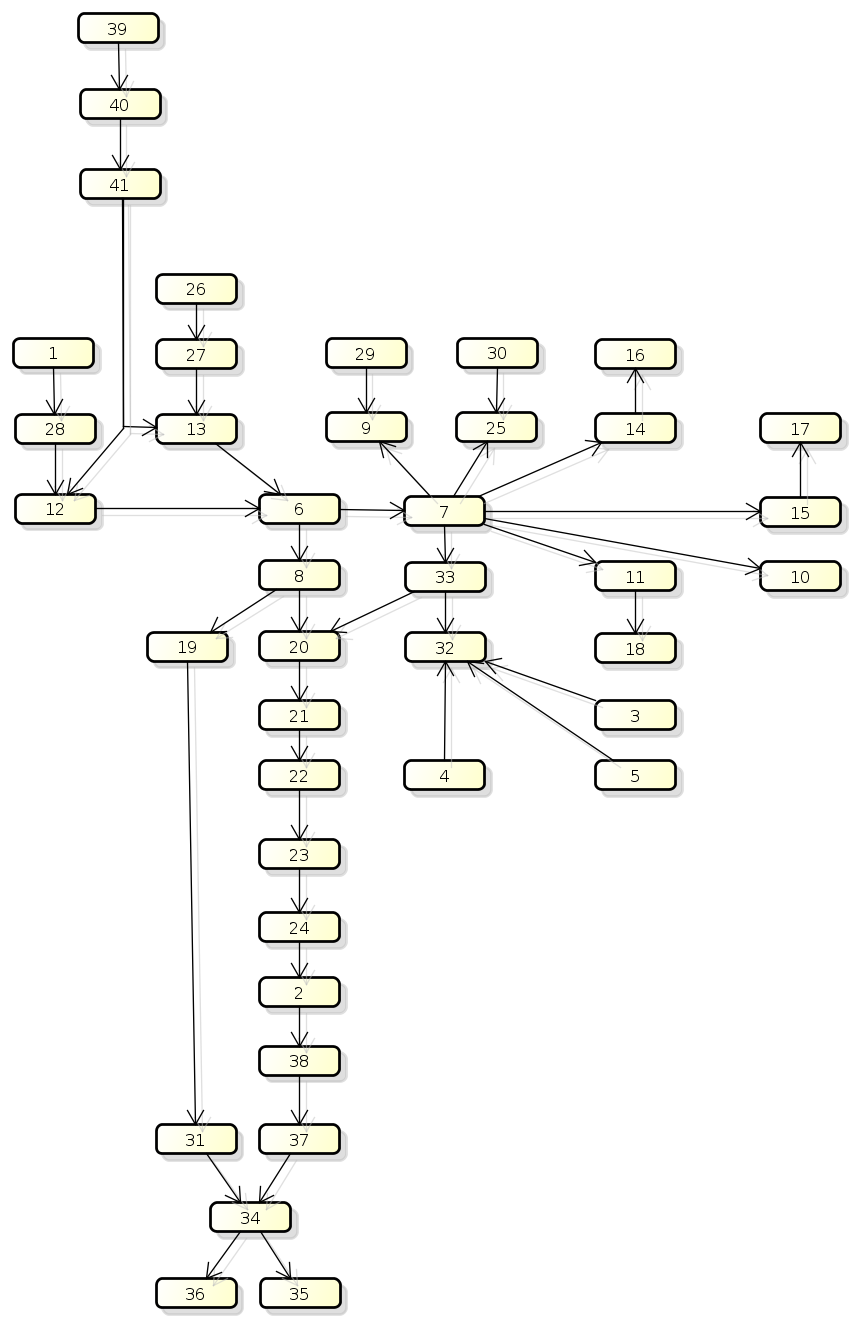
\includegraphics[scale=0.6]{image/process_vishnu.png}
\caption{Overview of the processes}
\end{figure}

Dans le process, on suppose que les étapes 39, 40 et 41 ne sont à faire que la première fois, 
et qu'il n'est pas nécessaire de les refaire dans les process suivants. Ainsi ils ne seront 
pas répétés mais sont quand même supposés en prérequis.
Vu la densité des éléments sur le schémas, il faut bien faire attention au sens qui sont 
indiqués par les flèches.

\section{Détail de chaque étape}

\subsection{1 - Mise à jour des fichiers STB astah}
Les fichiers STB astah se trouvent dans vishnu\_1/core/spec/stb. Ils contiennent les spécifications
techniques du besoin, c'est à dire les besoin du logiciel (dépendance logicielles et
matérielles pour fonctionner). Ils décrivent également les besoin attendus en sécurité et 
performance.

\subsection{2 - Implémenter la couche WS}
Dans le dépot eclipse\_1/WSAPI/src/main/java/com/sysfera/vishnu/api se trouve les 4 modules.
Dans chaque module se trouvent plusieurs dossiers importants:
\begin{itemize}
\item impl: Contient l'implémentation faisant le lien entre le JNI et le code WSDL.
\item data: Couche ajoutée pour faire le lien entre les énums EMF et les vrais classe d'énum. Une classe est à implémenter pour chaque énum défini dans le modèle.
\item test: Contient les tests JUnit de l'API WS.
\item A la racine du module se trouvent les classes JAVA générées à partir du WSDL du module en question.
\end{itemize}
Pour plus d'informations sur ces éléments, il faut se reporter au document décrivant le processus de mise à jour des WS.

\subsection{3 - Mise à jour du fichier astah archi}
Dans le dépot vishnu\_1/<module>/design se trouve un fichier Archi.asta décrivant l'architecture du module.
Toute modification de l'architecture d'un module doit être consignée dans ce document.

\subsection{4 - Mise à jour du fichier astah design}
Dans le dépot vishnu\_1/<module>/design se trouve un fichier Design.asta décrivant les classes du module
et leurs intéractions, ainsi que les liens fonctionnels entre les blocs clients/servers.
Tout ajout de classe (coté client et serveur) doit être mise dans ce document.

\subsection{5 - Mise à jour du fichier astah data}
Dans le dépot vishnu\_1/<module>/design se trouve un fichier data.asta décrivant les objets du module
et leurs intéractions. \\
\textbf{utilité ? Redondance avec ecore, voir pour supprimer ?}

\subsection{6 - Mise à jour de l'ecore }
Les fichiers ecore correspondent à la modélisation de tous les objets d'un module. Il se trouve dans
vishnu\_1/core/model, chaque module a son fichier ecore décrivant ses classes de données.
Se reporter au document dans \\
 vishnu\_1/core/process/doc/APIM2DB pour avoir un guide d'utilisation
pour créer, utiliser, manipuler, les ecore.

\subsection{7 - Mise à jour de l'apim }
Les fichiers APIM correspondent à la formalisation de l'API d'un module. Ainsi, chaque apim
contient des services prenant un certain nombre de ports (=paramètres). Chaque module a
son fichier apim décrivant son API. Il se trouve dans vishnu\_1/core/model. 
Se reporter au document dans vishnu\_1/core/process/doc/APIM2DB pour avoir un guide d'utilisation
pour créer, utiliser, manipuler, les apim.

\subsection{8 - Utilisation de emf4cpp pour générer les classes de données C++ }
Les classes de données sont générées à partir du modèle ecore. Pour se faire il 
faut utiliser le script suivant emf4cpp.generator\_SF.sh, en lui donnant le
modèle ecore. Ce script se trouve dans:
vishnu\_1/core/deps/emf\_bin. \\
Attention à bien utiliser ce script qui est une version modifiée par SysFera 
du générateur de base.

\subsection{9 - Utilisation du générateur de documentation API}
Utilise le générateur com.sysfera.codegen.docbook.DocBookDocumentGenerator
issu du dépot eclipse\_1. Ce générateur prend 2 paramètres :
\begin{itemize}
\item \textit{-I <vishnu\_1>/core/model}: Le chemin complet de la racine au dépot 
vishnu\_1/core/model
\item \textit{<vishnu\_1>/core/specs/docbook/api-template.docbook}: Le chemin
complet jusqu'au fichier api-template.docbook situé dans le dépot vishnu\_1.
\end{itemize}
Ne pas oubliez de générer les pdf et html ensuite.

\subsection{10 - Utilisation du générateur de manpage}
Utilise le générateur com.sysfera.codegen.docbook.DocBookDocumentGenerator
issu du dépot eclipse\_1. Ce générateur prend 2 paramètres :
\begin{itemize}
\item \textit{-I <vishnu\_1>/core/model}: Le chemin complet de la racine au dépot 
vishnu\_1/core/model
\item \textit{<vishnu\_1>/<module>/doc/man/docbook/man<module>-template.docbook}:
 Le chemin complet jusqu'au fichier docbook template des manpages du module 
 concerné situé dans le dépot vishnu\_1.
\end{itemize}

\subsection{11 - Utilisation du générateur de wsdl}
Utilise le générateur com.sysfera.codegen.ws.Apim2WsdlGenerator issu du
dépot eclipse\_1. Ce générateur prend en paramètre un seul fichier, qui
est l'apim du module en question et génère le fichier /tmp/wsdl-gen.wsdl.
Il faut ensuite le renommer et le placer dans eclipse\_1/WSAPI/wsdl.

\subsection{12 - Utilisation du générateur de STB}
Utilise le générateur com.sysfera.codegen.docbook.DocBookDocumentGenerator
issu du dépot eclipse\_1. Ce générateur prend 2 paramètres :
\begin{itemize}
\item \textit{-I <vishnu\_1>}: Le chemin complet de la racine au dépot 
vishnu\_1
\item \textit{<vishnu\_1>/core/specs/docbook/STB-template.docbook}:
 Le chemin complet jusqu'au fichier STB-template.docbook
 situé dans le dépot vishnu\_1.
\end{itemize}
Ne pas oubliez de générer les pdf et html ensuite.

\subsection{13 - Utilisation du générateur de Spec générales}
Utilise le générateur com.sysfera.codegen.docbook.DocBookDocumentGenerator
issu du dépot eclipse\_1. Ce générateur prend 2 paramètres :
\begin{itemize}
\item \textit{-I <vishnu\_1>}: Le chemin complet de la racine au dépot 
vishnu\_1
\item \textit{<vishnu\_1>/core/specs/docbook/SpecGen-template.docbook}:
 Le chemin complet jusqu'au fichier SpecGen-template.docbook
 situé dans le dépot vishnu\_1.
\end{itemize}
Ne pas oubliez de générer les pdf et html ensuite.

\subsection{14 - Mise à jour du userman}
Il faut mettre à jour le fichier dans le dépot vishnu\_1
core/doc/userman/docbook/userman-template.docbook. Ne pas oubliez
de mettre à jour l'en-tête pour indiquer les modifications apportées
au document.

\subsection{15 - Mise à jour de l'adminman}
Il faut mettre à jour les fichiers core/doc/adminman/docbook/adminman-template.docbook
 et \\
 core/doc/adminman/docbook/adminman\_eng-template.docbook qui correspondent
à la version Française et Anglaise du guide de l'administrateur VISHNU.
Ne pas oubliez de mettre à jour l'en-tête pour indiquer les modifications 
apportées au document.

\subsection{16 - Génération du userman}
Utilise le générateur com.sysfera.codegen.docbook.DocBookDocumentGenerator
issu du dépot eclipse\_1. Ce générateur prend 2 paramètres :
\begin{itemize}
\item \textit{-I <vishnu\_1>/core/model}: Le chemin complet de la racine au dépot 
vishnu\_1/core/model
\item \textit{<vishnu\_1>/core/doc/usermanual/docbook/userman-template.docbook}:
 Le chemin complet jusqu'au fichier userman-template.docbook
 situé dans le dépot vishnu\_1.
\end{itemize}
Ensuite exécuté le script \textit{update\_files.sh} qui génère les versions
pdf et html à jour.

\subsection{17 - Génération des adminman}
Utilise le générateur com.sysfera.codegen.docbook.DocBookDocumentGenerator
issu du dépot eclipse\_1. Ce générateur prend 2 paramètres :
\begin{itemize}
\item \textit{-I <vishnu\_1>/core/model}: Le chemin complet de la racine au dépot 
vishnu\_1/core/model
\item \textit{<vishnu\_1>/core/doc/adminmanual/docbook/adminman-template.docbook}:
 Le chemin complet jusqu'au fichier adminman-template.docbook
 situé dans le dépot vishnu\_1.
\item Ou (pour la version Anglaise) \textit{<vishnu\_1>/core/doc/adminmanual/docbook/adminman\_eng-template.docbook}:
 Le chemin complet jusqu'au fichier adminman\_eng-template.docbook
 situé dans le dépot vishnu\_1.
\end{itemize}
Ensuite exécuter le script \textit{update\_files.sh} qui génère les versions
pdf et html à jour pour les versions Anglaise et Française.

\subsection{18 - Génération de la doc WS à partir des WSDL}
Il faut exécuter la commande suivante depuis le dossier vishnu\_1/core/tools/docWS (ou module est à remplacer par le nom du module):\\
xsltproc --param ignore.image.scaling 1 wsdl-viewer.xsl <path>/module.wsdl > module.html \\
Pour générer le pdf correspondant au html ainsi créé :
htmldoc -f UMS.pdf UMS.html

\subsection{19 - Mise à jour du plan du test}
Pour chaque module, un plan de test est écrit avant l'implémentation
du module. En parallèle du codage, les tests décrits seront implémentés,
et à la fin du codage, on vérifiera que le code produit passe bien
le plan de test. \\
Les plans de test sont dans vishnu\_1/<module>/test/testPlan. Il faut modifier
l'odt puis générer le docbook issu de l'odt puis les pdf/html issus du docbook.

\subsection{20 - Codage C++ des clients/serveurs}
Réalisation du code métier, à faire en suivant l'architecture existante.

\subsection{21 - Mise à jour des mappers}
Pour historiser et retrouver les commandes tappées dans une session précédente,
le code contient un système de 'mappers' dans core/src/registry. Chaque module
a son mapper associé et pour chaque fonction, il faut implémenter sa fonction
de reconnaissance et lui associer son code. Toute modification d'API, ou
d'objets dans les API impacte le mapper.
Un document a été commencé au sujet du mapper mais n'est pas encore fini.
En cas de doute, se référer si possible à Eugène ou Kevin (plutôt le second).

\subsection{22 - Eventuellement, mettre à jour les exporteurs (pas si uniquement shell)}
VISHNU possède une fonctionnalité d'export des commandes historisées, et de
manière similaire aux mappers, si un autre export que le shell est défini,
il faut mettre à jour les exporteurs dans vishnu\_1/IMS/src/server/data/export.
Actuellement seul shell est disponible mais ce ne sera potentiellement pas
toujours le cas.

\subsection{23 - Modifier le fichier swig (vishnu.i)}
Dans vishnu\_1/swigAPI/vishnu.i se trouve la définition du mapping pour swig
à la fois pour le python et pour les WS. Toute modification d'API, ajout 
d'objets, ajout d'exception, ajout de module doit avoir le mapping
correspondant ajouté dans ce fichier.

\subsection{24 - Compiler avec swig/java/python pour générer les fichiers de generated}
Dans vishnu\_1/swigAPI se trouve un dossier generated contenant les parties 
python et WS déjà générées avec 'notre bon swig', cela fait que le client
peut compiler les WS et python sans swig mais en utilisant le code déjà 
généré. Il faut mettre à jours ces fichiers à chaque mise à jour du fichier
vishnu.i.

\subsection{25 - Utilisation du générateur de documentation CLI}
Utilise le générateur com.sysfera.codegen.docbook.DocBookDocumentGenerator
issu du dépot eclipse\_1. Ce générateur prend 2 paramètres :
\begin{itemize}
\item \textit{-I <vishnu\_1>/core/model}: Le chemin complet de la racine au dépot 
vishnu\_1/core/model
\item \textit{<vishnu\_1>/core/specs/docbook/cli-template.docbook}: Le chemin
complet jusqu'au fichier cli-template.docbook situé dans le dépot vishnu\_1.
\end{itemize}
Ne pas oubliez de générer les pdf et html ensuite.

\subsection{26 - Mise à jour du fichiers astah *MS}
Chaque module a son fichier module.asta qui correspond aux spécifications du 
module avec la définition des uses cases et leur description, les requirements
ayant amené à la constitution du module, etc ...

\subsection{27 - Mise à jour du fichiers SpecGen-template}
Il faut mettre à jour le fichier dans le dépot vishnu\_1
core/spec/docbook/SpecGen-template.docbook. Ne pas oubliez
de mettre à jour l'en-tête pour indiquer les modifications apportées
au document. Ce fichier défini les spécifications générales de VISHNU.

\subsection{28 - Mise à jour du fichiers STB-template}
Il faut mettre à jour le fichier dans le dépot vishnu\_1
core/spec/docbook/STB-template.docbook. Ne pas oubliez
de mettre à jour l'en-tête pour indiquer les modifications apportées
au document. Ce fichier défini les besoins de VISHNU.

\subsection{29 - Mise à jour du fichiers api-template}
Il faut mettre à jour le fichier dans le dépot vishnu\_1
core/spec/docbook/api-template.docbook. Ne pas oubliez
de mettre à jour l'en-tête pour indiquer les modifications apportées
au document. Ce fichier défini toutes les API de VISHNU.

\subsection{30 - Mise à jour du fichiers cli-template}
Il faut mettre à jour le fichier dans le dépot vishnu\_1
core/spec/docbook/cli-template.docbook. Ne pas oubliez
de mettre à jour l'en-tête pour indiquer les modifications apportées
au document. Ce fichier défini l'API CLI de VISHNU.

\subsection{31 - Codage C++ des tests}
Dans vishnu\_1/<module>/test/src se trouve des boost tests. A chaque nouvelle
fonctionnalité, bug, etc ... il faut mettre à jour les tests. Ces tests sont
exécutés quotidiennement sur le serveur d'intégration continu hudson.

\subsection{32 - Générer le fichier design d'un module}
Utilise le générateur com.sysfera.codegen.docbook.DocBookDocumentGenerator
issu du dépot eclipse\_1. Ce générateur prend 2 paramètres :
\begin{itemize}
\item \textit{-I <vishnu\_1>}: Le chemin complet de la racine au dépot 
vishnu\_1/
\item \textit{<vishnu\_1>/<module>/design/docbook/<module>Design-template.docbook}:
 Le chemin complet jusqu'au fichier design du module en question
 situé dans le dépot vishnu\_1.
\end{itemize}
Ne pas oubliez de générer les pdf et html ensuite.


\subsection{33 - Création du fichier apim internal}
Les apim correspondent aux API externes visibles par les clients.
Lorsque nos services communiquent, ces api visibles ne sont pas celles
que l'on utilise en interne entre le client et le serveur. Le fichier
<module>\_Internal.apim permet de spécifier pour chaque module l'interface 
utilisée entre le client et le serveur.
Ces fichiers sont dans vishnu\_1/core/model

\subsection{34 - Passer les tests}
Il faut passer le plan de test.

\subsection{35 - Ecrire le rapport de test}
Ecrire le rapport de test reprenant point par point tout les tests définis
dans le plan de test et indiquant si les tests ont réussis ou non.
Ces tests sont mis dans \\
vishnu\_1/<module>/test/testReports/report<module>Test.docbook. Il faut
écrire le rapport directement en docbook.
Ne pas oubliez de générer les pdf et html ensuite.

\subsection{36 - Intégrer les tests en test automatiques hudson}
Afin de valider quotidiennement qu'il n'y a pas de régression, il faut 
intégrer les tests à la plateforme de tests continus hudson mise en 
place dans les VM sur graal.

\subsection{37 - Regénérer les jars}
L'utilisation du script de release permet de regénérer les jars pour les mettre
dans \\
 eclipse\_1/WSAPI/WSAPI.jar et ecplise\_1/VishnuLib/VishnuLib-1.0-SNAPSHOT.jar

\subsection{38 - Mettre les fichiers swig java dans les jars du dépot eclipse}
Quand on a regénéré les fichiers java avec swig lors de la compilation de 
vishnu\_1, il faut les mettre dans \\
 eclipse\_1/VishnuLib/src/main/java/com/sysfera/vishnu/api/vishnu/internal.

\subsection{39 - Récupérer les dépots GIT}
A ne faire qu'une fois au tout début: \\
git clone <login>@graal.ens-lyon.fr:/home/GIT/SysFera/repositories/eclipse\_1.git \\
git clone <login>@graal.ens-lyon.fr:/home/GIT/SysFera/repositories/vishnu\_1.git

\subsection{40 - Configurer son eclipse pour supporter les ecore/apim}
Voir le document dans vishnu\_1/core/process/doc/APIM2DB

\subsection{41 - Récupérer les projets dans le workspace les projets dans eclipse\_1}
Voir le document dans vishnu\_1/core/process/doc/APIM2DB, importer les projets.%%%%%%%%%%%%%%%%%%%%%%%%%%%%%%%%%%%%%%%%%%%%%%%%%%
%% SECTION APIM
%%%%%%%%%%%%%%%%%%%%%%%%%%%%%%%%%%%%%%%%%%%%%%%%%%

\end{document}
